Finalmente presentamos en este último punto las simulaciones realizadas sobre el experimento. Estas han sido desarrolladas mediante un código bastante avanzado sobre el que se han realizado una serie de modificaciones. Su finalidad es simular un prototipo del detector rectílineo a diferencia del nuestro, que presenta forma de U. Una imagen transversal del prototipo puede verse en la figura~\ref{imagenprototiposimulado}.

\begin{figure}[hbtp]
\centering
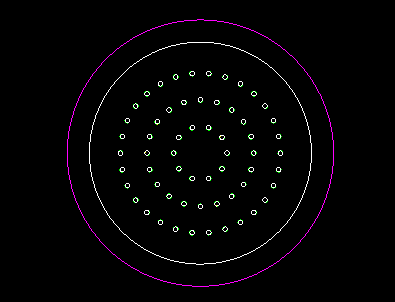
\includegraphics[scale=0.4]{Finalforntal.png}
\caption{Imagen transversal del prototipo\label{imagenprototiposimulado}}
\end{figure}

Está formado por un cilindro externo de teflón  de radio interno $2.5~\cm$, $0.5~\cm$ de grosor y una longitud de $80~\cm$ dando lugar a un volumen interno de $1.1781~l$. En su interior residen 60 fibras centelleaoras, dispuestas formando 3 círculos según la figura~\ref{imagenprototiposimulado}. El círculo interno, con un diámetro de $6~\mm$, contiene 10 fibras, el círculo intermedio, con un diámetro de $12~\mm$, contiene 20 fibras y el círculo externo, con un diámetro de $18~\mm$ contiene 30 fibras. El volumen efectivo interno (descontando el volumen ocupado por las fibras) es de $1.1498~\liter$, volumen que en la práctica será ocupado por el agua tritiada.

Las fibras que se han simulado pretenden ser las utilizadas hasta el momento, fibras centelleadoras BCF-12 de $1~\milli\meter$ de diámetro pero con longitud de $60~\centi\meter$. En los $20~\cm$  del cilindro de teflón que no están ocupados por las fibras centelleadoras (10 cm a cada lado) se pretende situar los PMTs o, en su defecto, los SiPMs para detectar los fotones que se reciban de las fibras. Ambos lados están separados por una ventana de cuarzo que permita el paso de los fotones y no del agua destilada, ya que ninguno de los fotosensores que utilizarán en este experimento puede encontrarse en contacto con el agua en ningún momento.

La simulación describe la emisión de una fuente de tritio que en la práctica se encontrará cubriendo por completo el volumen libre del interior del cilindro de teflón pero, con el objetivo de agilizar las simulaciones, sólo ha sido necesario implementar un interior de aire y unos cilindros de agua tritiada de $50~\micro\meter$ de grosor alrededor de cada fibra centelleadora. Debido a que el recorrido libre medio de los electrones en el agua es $5~\micro\meter$ ambas situaciones son análogas. 

Hay que tener en cuenta que los resultados presentados de estas simulaciones únicamente describen los electrones detectados en las fibras y la posterior conversión de estos en fotones. En esta simulación no se ha implementado el posterior tratamiento de la luz, por lo que todavía no podemos justificar la importancia de la pérdida de luz discutida en la seccion~\ref{sec:Resultados}.

Los resultados obtenidos para una simulación de $10000$ eventos se muestran a continuación:
\begin{enumerate}
\item{} En primer lugar se ha realizado un histograma energético de los electrones emitidos en la desintegración del tritio, el cual se muestra en la figura~\ref{espectrotritiosimuladonewpage}.

\begin{figure}[hbtp]
\centering
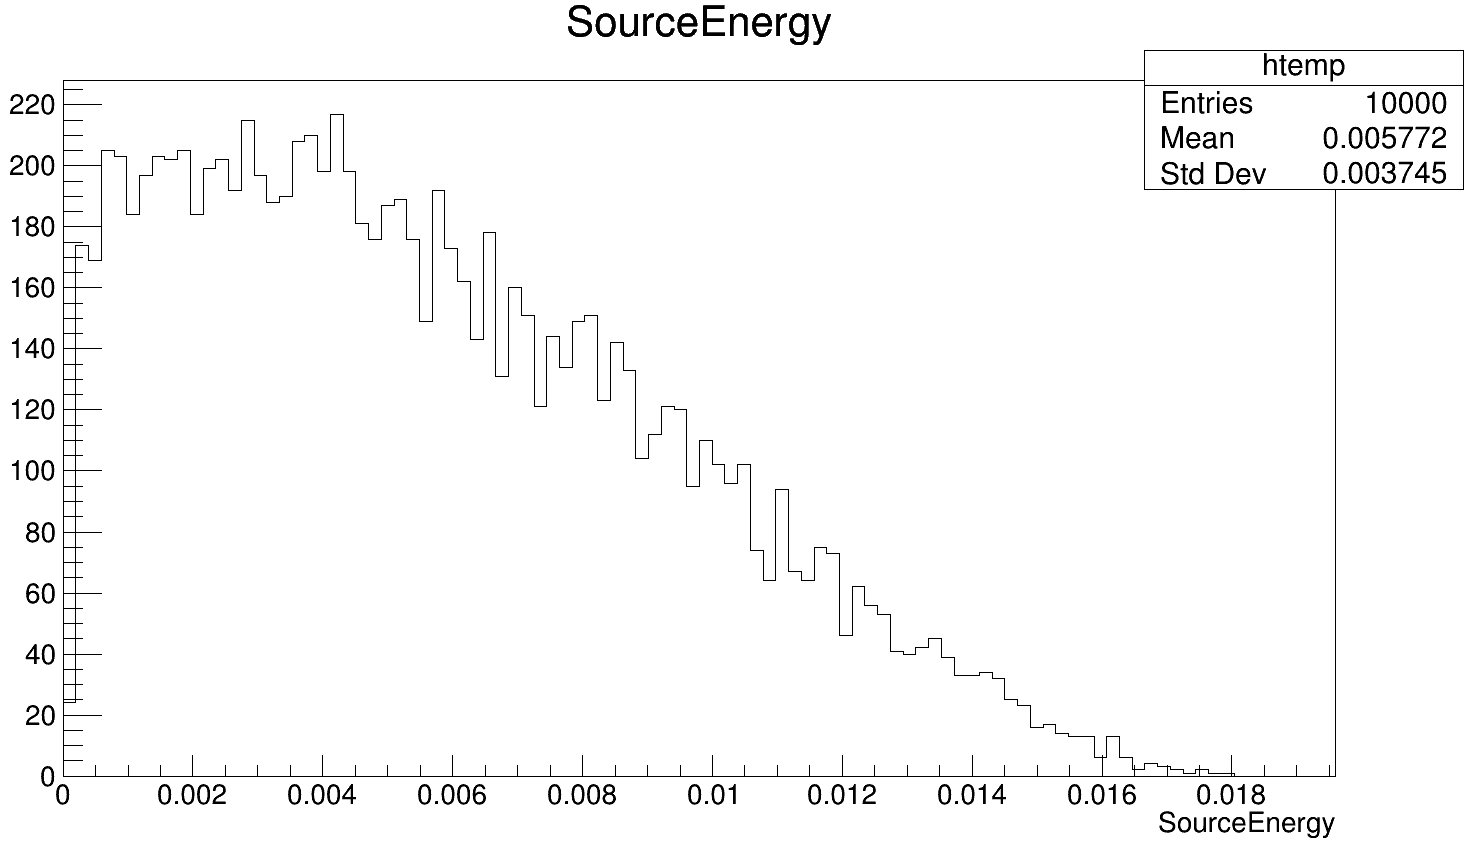
\includegraphics[scale=0.2]{espectrotritiosimulado.png}
\caption{Espectro simulado de los electrones procedentes de la desintegración del tritio (Escala en MeV)\label{espectrotritiosimuladonewpage}}
\end{figure}

Podemos ver que se trata de un espectro que se ajusta perfectamente al espectro teórico, fig.~\ref{fig:Espectrotritio}. Para conseguir un espectro más suave será necesario realizar una simulación con un mayor número de eventos, para lo cual será necesario acceder a uno de los centros  de cálculo disponibles para disponer de de una mayor potencia de computación.

\item{} Seguidamente, se realizó un histograma de la posición de la fibra en la cual se había detectado el suceso. Este se muestra en la  figura~\ref{espectroespacial}, en la que se muestran tres imágenes asociadas a cada uno de los ejes espaciales.

\begin{figure}[htb]
\centering
{
%\subfloat[Espectro de emisión]
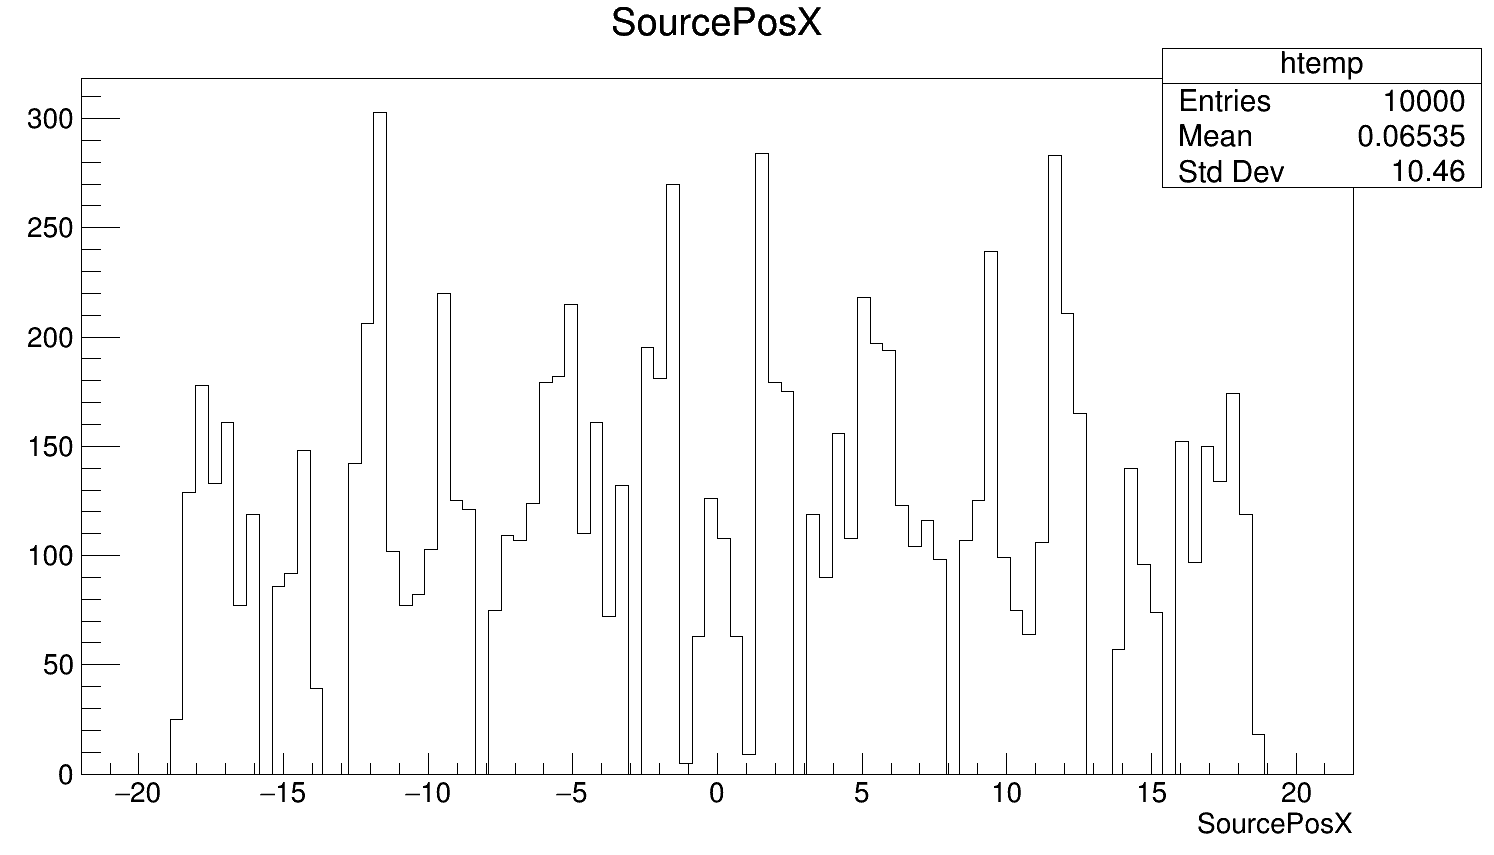
\includegraphics[scale=0.1]{eventosXfibras.png} 
}
{
%\subfloat[Espectro de emisión]
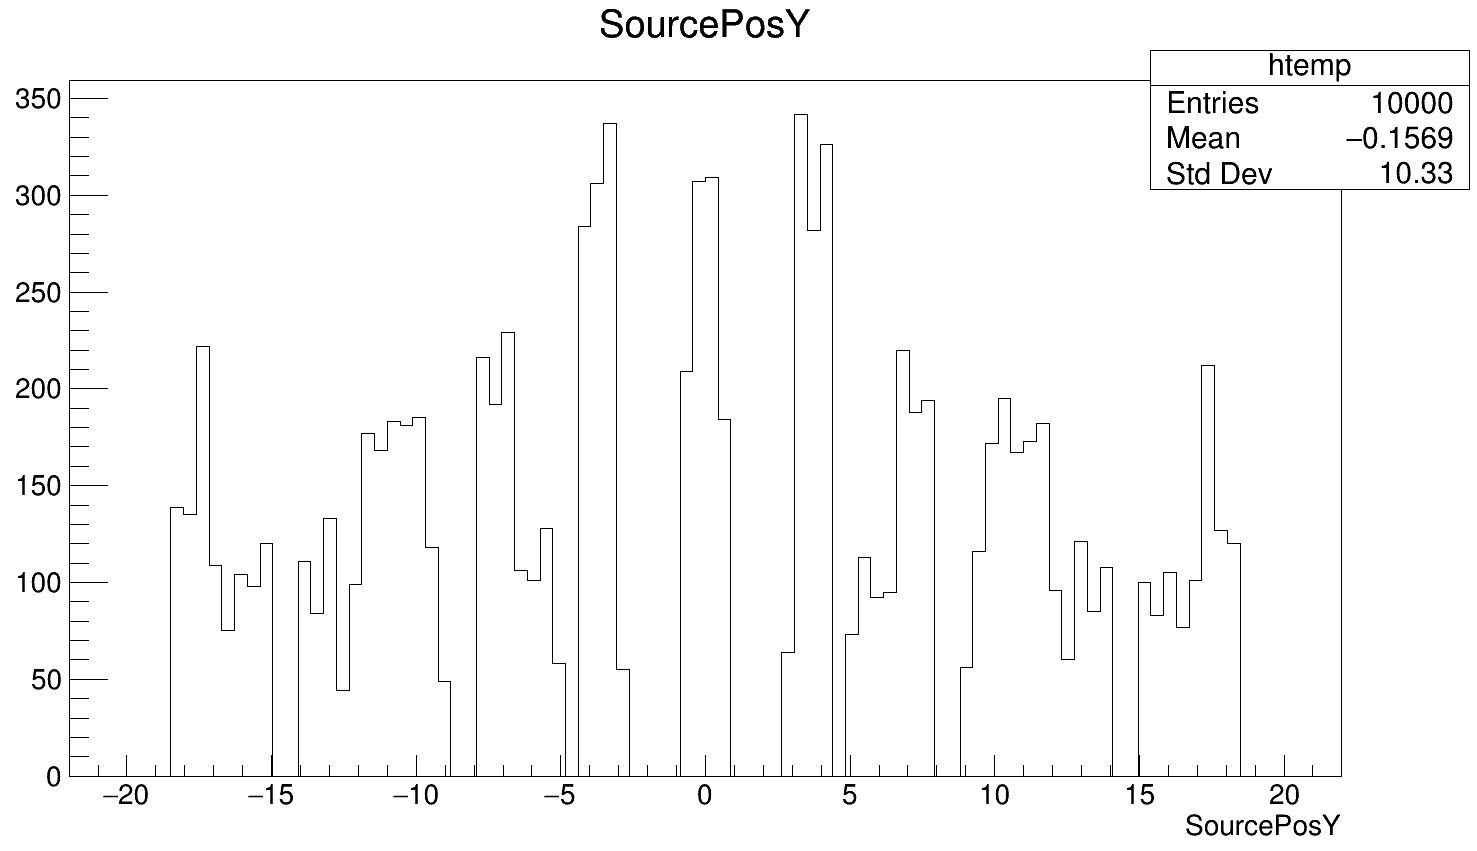
\includegraphics[scale=0.1]{eventosYfibras.png} 
}
{
%\subfloat[Espectro de emisión]
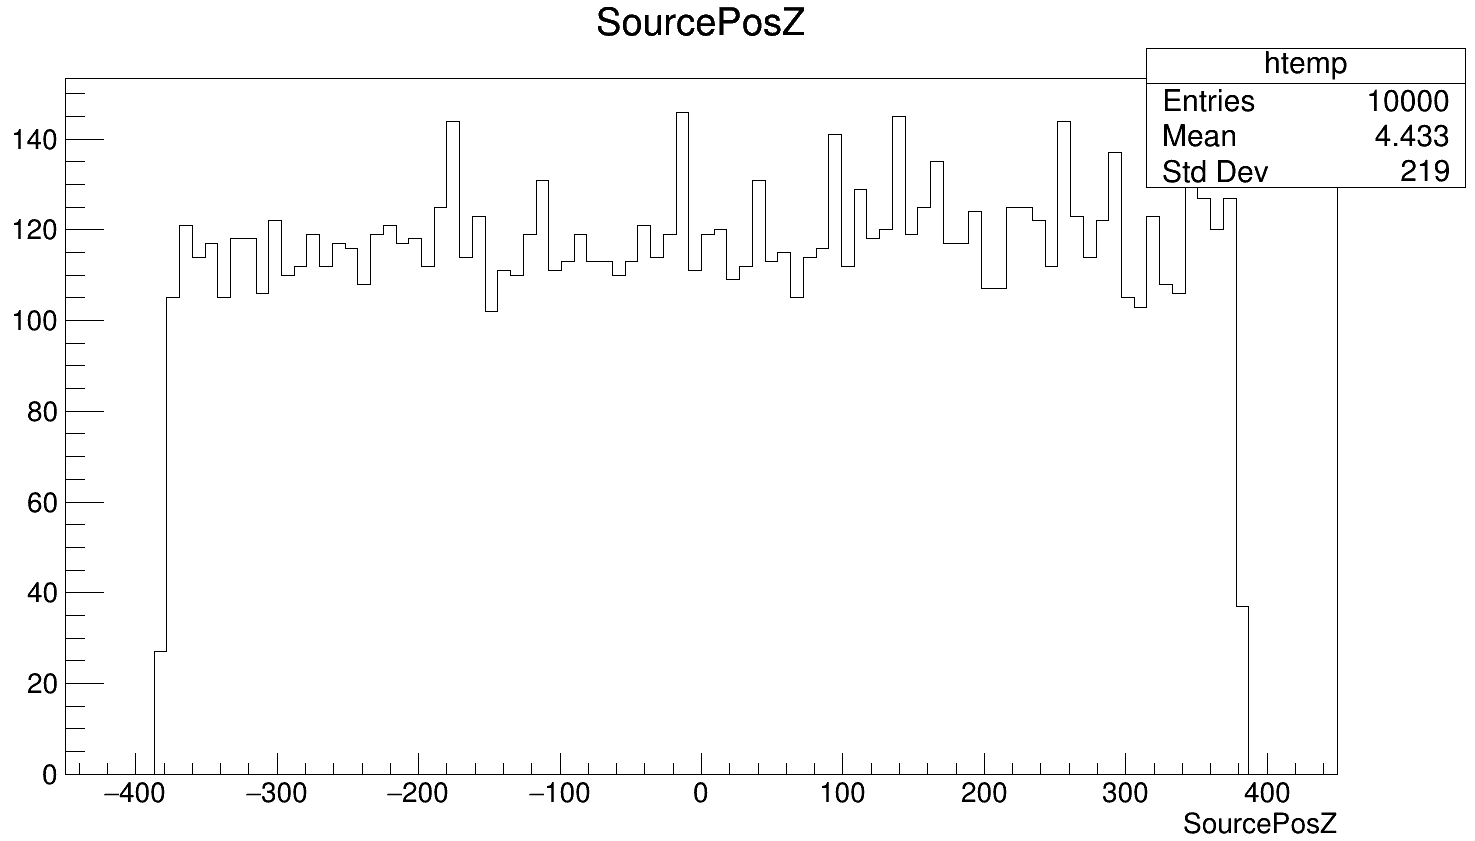
\includegraphics[scale=0.1]{eventosZfibras.png} 
}
\caption{Histograma espacial de la posición de detección de los electrones en las fibras\label{espectroespacial}}
\end{figure}

En los ejes X e Y puede apreciarse una detección más o menos uniforme en los puntos espaciales donde se encuentran situadas las fibras y, en el eje Z puede apreciarse una detección totalmente uniforme a lo largo de la longitud de las fibras. Este es un resultado que deberíamos esperar ya que se ha simulado una fuente de actividad uniforme y constante en el tiempo.

\item{} Se ha asignado un número del 1 al 60 a cada una de las fibras y se ha realizado un histograma del número de eventos que se han detectado en cada una de ellas. Este se muestra en la figura~\ref{sucesossobrecadafibra}.

\begin{figure}[hbtp]
\centering
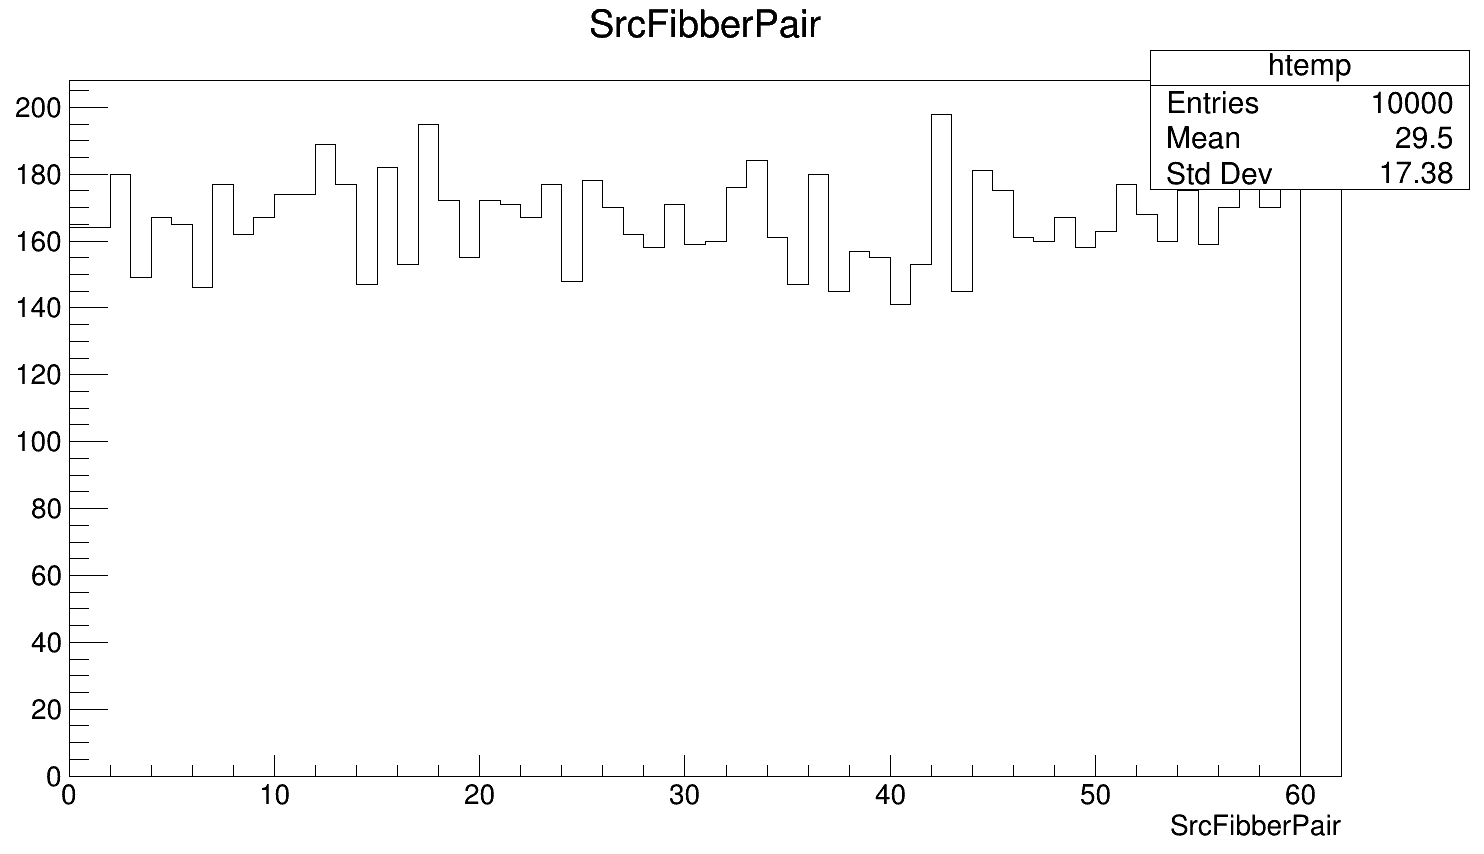
\includegraphics[scale=0.2]{Histogramafibras.png}
\caption{Histograma de sucesos sobre cada fibra\label{sucesossobrecadafibra}}
\end{figure}

Podemos observar de nuevo que se trata de una deposición uniforme sobre las fibras. Todas han detectado aproximadamente el mismo número de eventos, algo que de nuevo deberíamos esperar.

\item{} Seguidamente se ha obtenido el espectro de energía depositada en el agua y en las fibras, además de las longitudes recorridas en ambos medios por los electrones del tritio. Ambas se muestran en las figuras~\ref{deposicionagua} y \ref{deposicionfibras}, respectivamente

\begin{figure}[htb]
\centering
{
%\subfloat[Espectro de emisión]
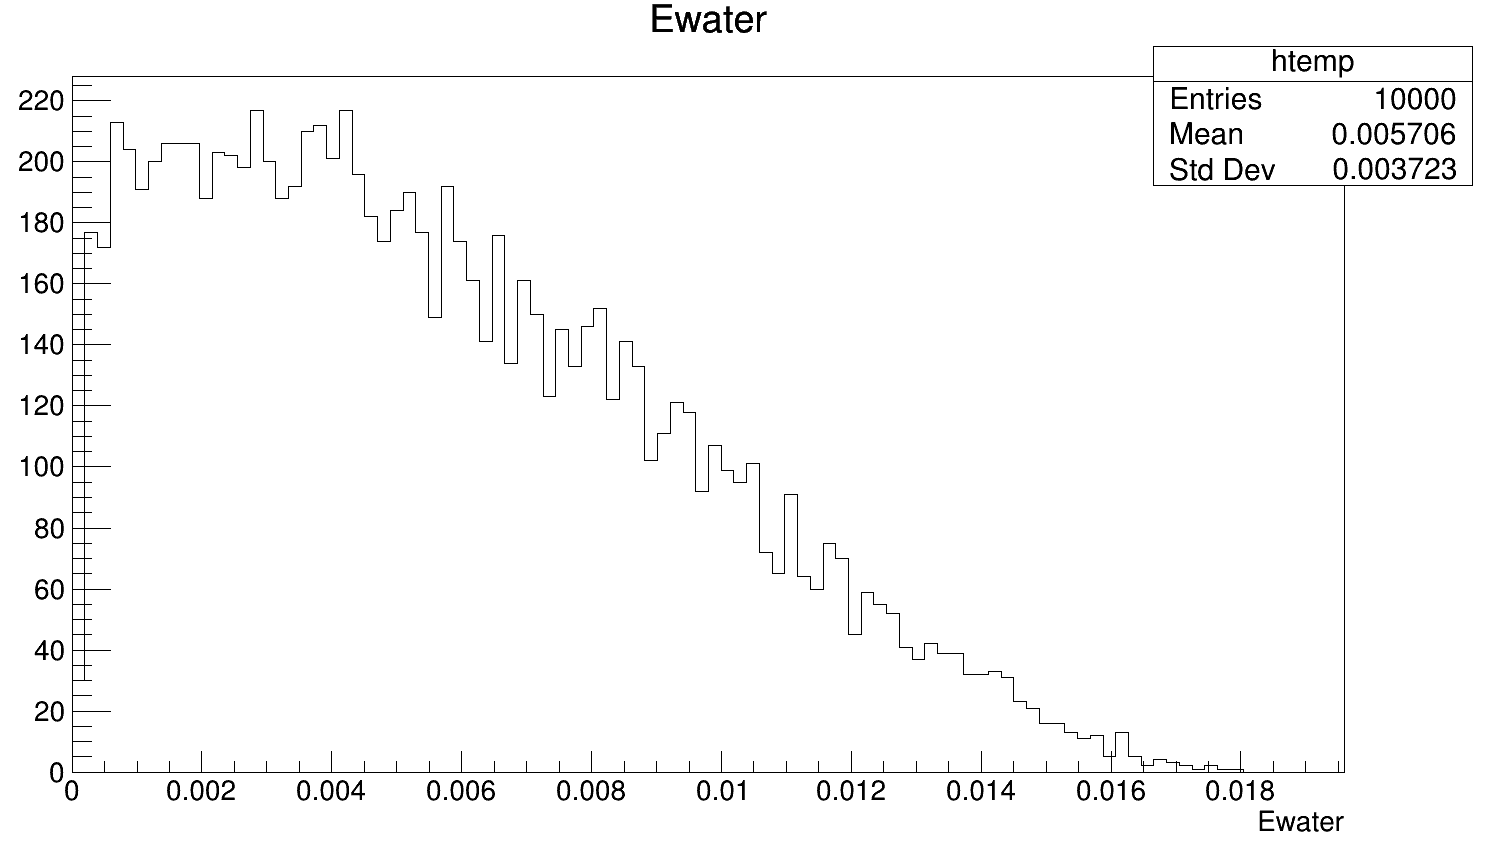
\includegraphics[scale=0.1]{deposicionenergiaagua.png} 
}
{
%\subfloat[Espectro de emisión]
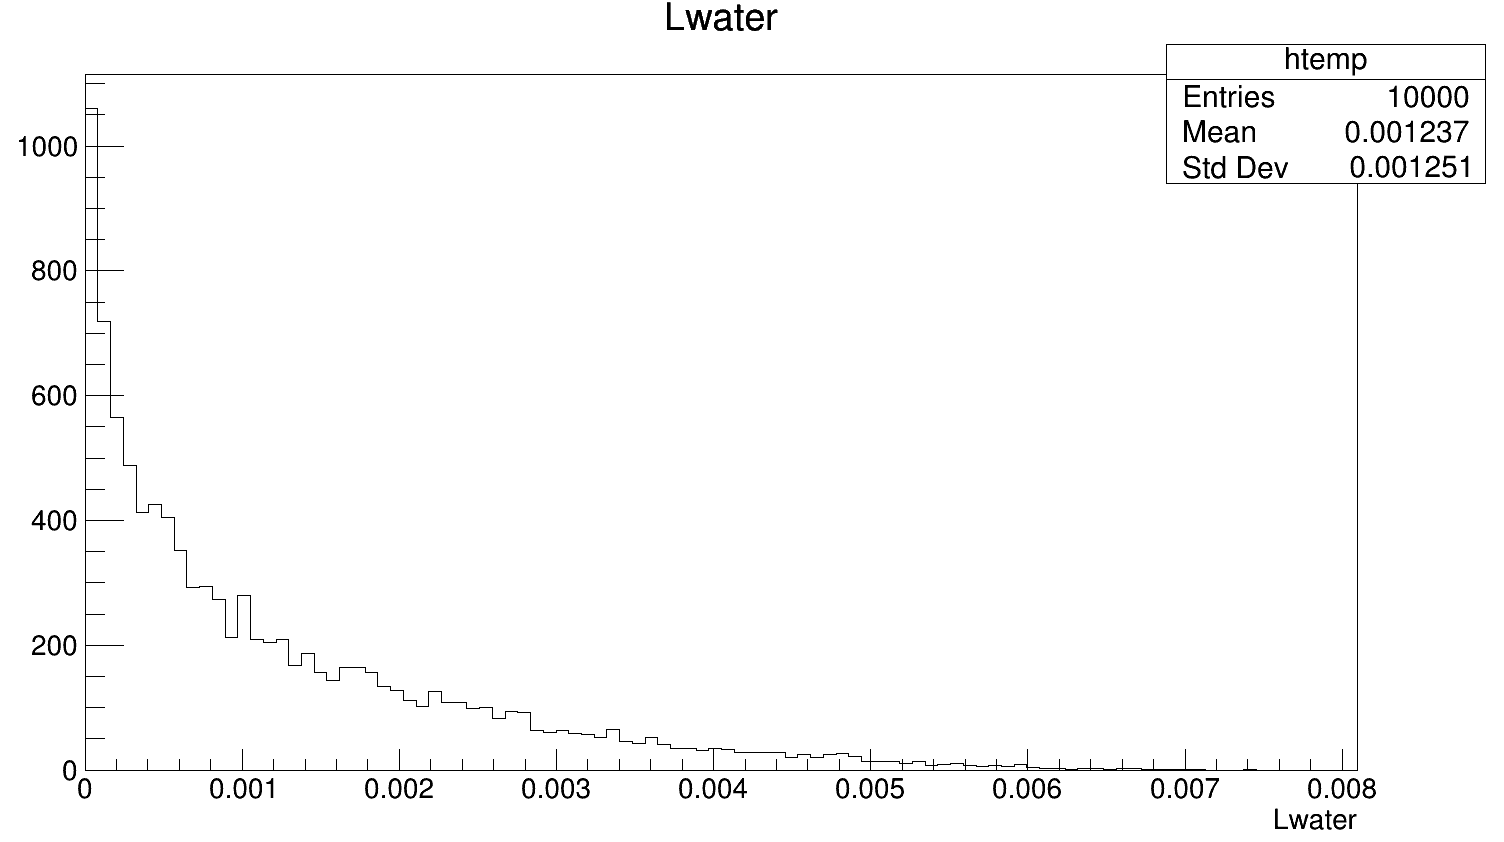
\includegraphics[scale=0.1]{longitudrecorridaagua.png} 
}
\caption{Histograma energético y espacial de los electrones absorbidos en al agua\label{deposicionagua}}
\end{figure}

\begin{figure}[htb]
\centering
{
%\subfloat[Espectro de emisión]
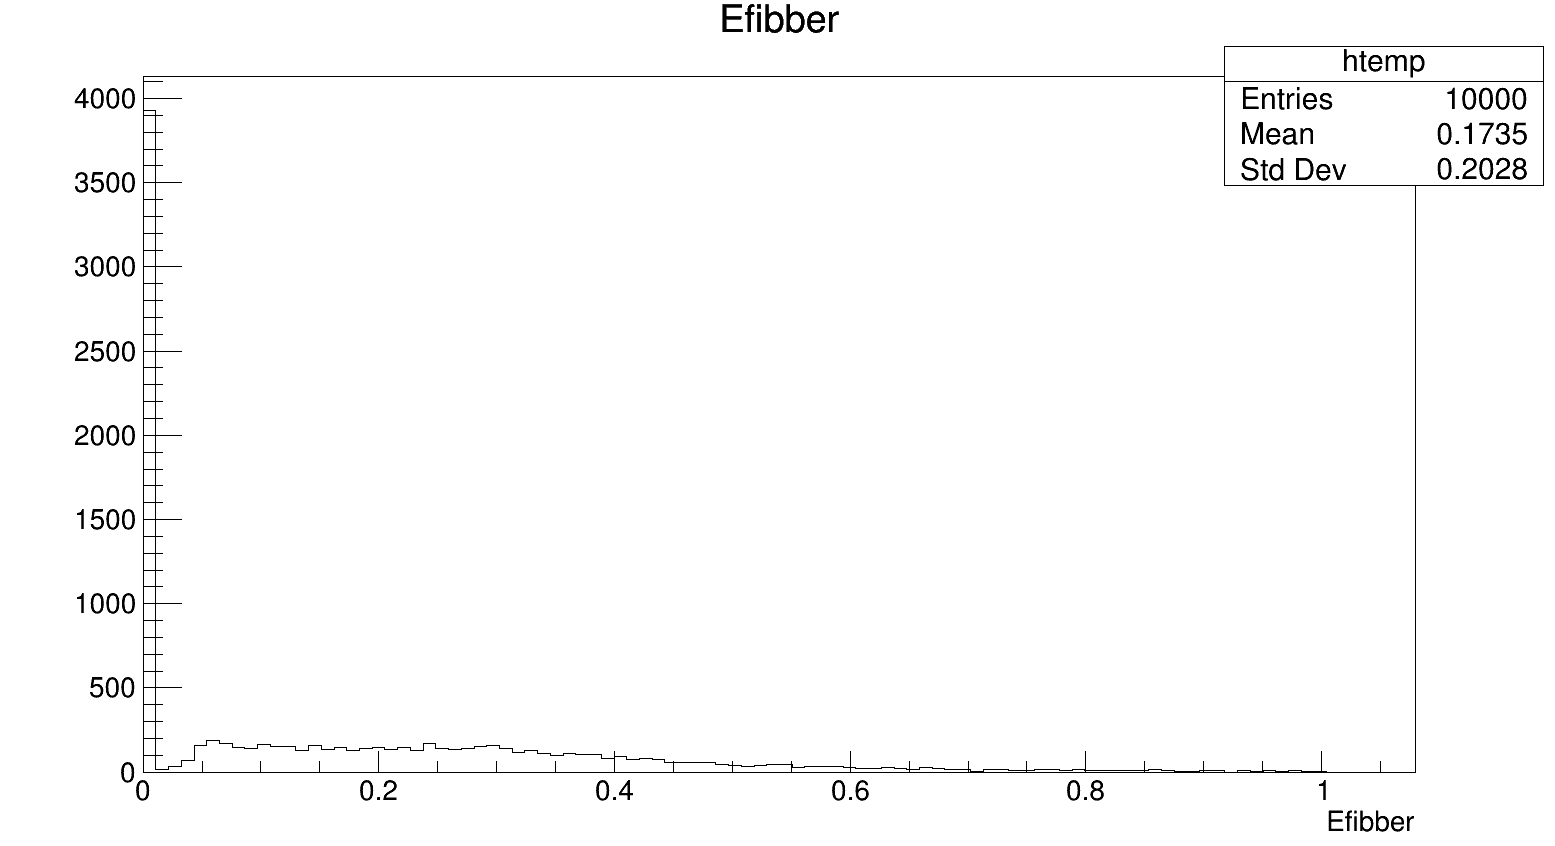
\includegraphics[scale=0.1]{energiadeposicionfibras.png} 
}
{
%\subfloat[Espectro de emisión]
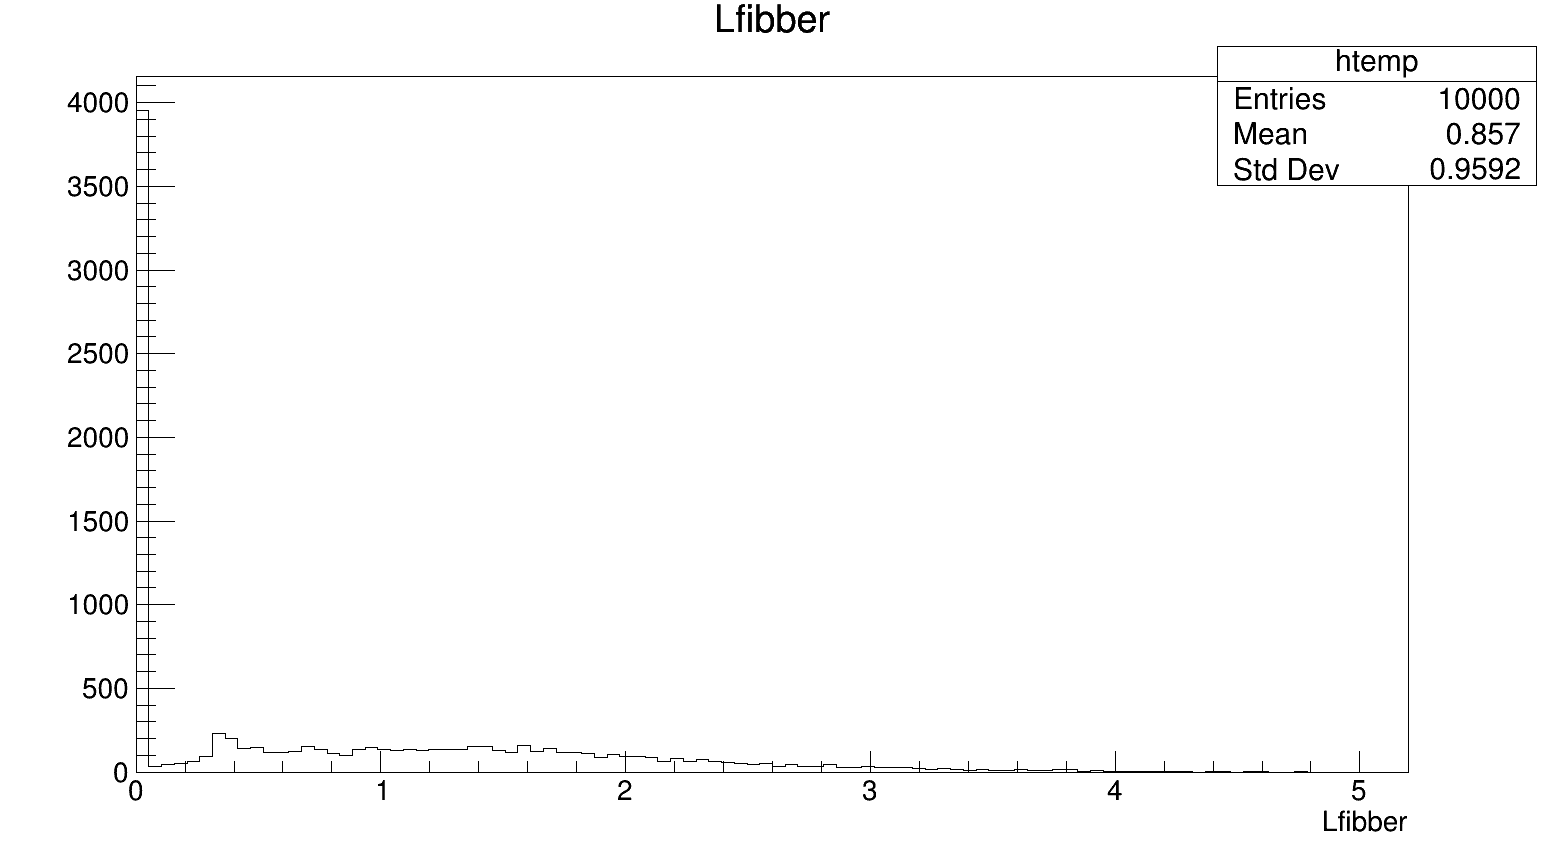
\includegraphics[scale=0.1]{longitudfibras.png} 
}
\caption{Histograma energético y espacial de los electrones absorbidos en las fibras\label{deposicionfibras}}
\end{figure}

En la figura~\ref{deposicionagua} podemos observar que la energía depositada presenta un espectro típico de una desintegración $\beta$ y la longitud recorrida por los electrones presenta una atenuación exponencial, función que, teóricamente, describe el fenómenos de atenuación, $N=N_0\exp{(-x/\lambda)}$.

Podemos observar por tanto que el programa esta simulando correctamente la absorción de tritio en el agua. Algo similar ocurre en la figura~\ref{deposicionfibras}, pero en estos histogramas no puede apreciarse debido a limitaciones que presenta el código desarrollado.

\item{} Finalmente se ha obtenido un histograma del número de fotones producidos en cada detección del tritio. Este se muestra en la figura~\ref{reemision}.

\begin{figure}[hbtp]
\centering
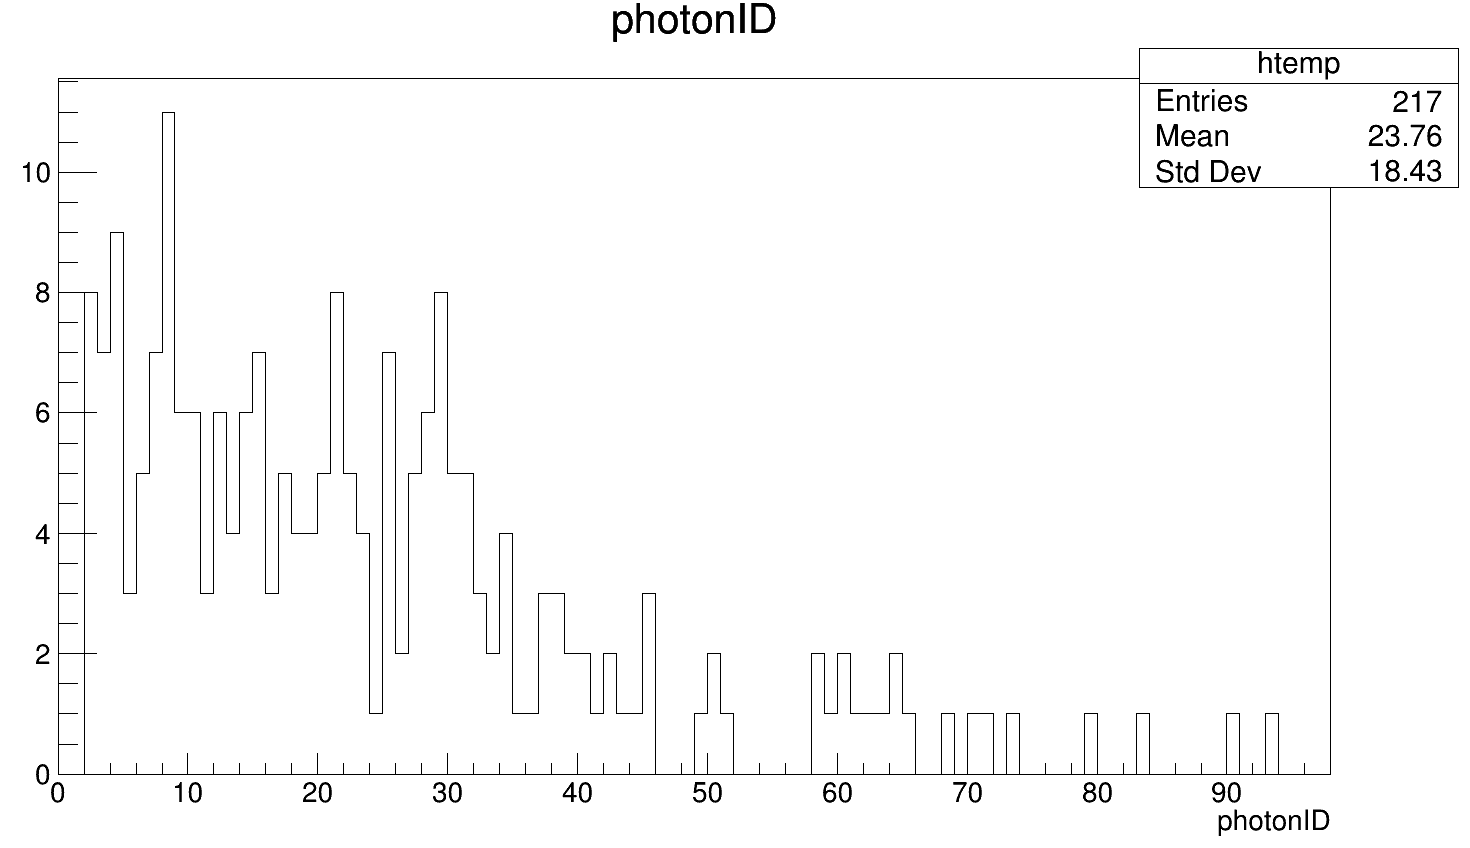
\includegraphics[scale=0.2]{reemisionfotones.png}
\caption{Histograma del número de fotones reemitidos en una detección \label{reemision}}
\end{figure}

Dado que existe una equivalencia entre la energía de la partícula detectada en la fibra y el número de fotones que esta reeemite, deberíamos esperar un espectro similar a una desintegración $\beta$, fig.~\ref{fig:Espectrotritio}. Podemos observar que, efectivamente, se cumple.

Hay que tener en cuenta que sólo han sido detectados y transformados en luz 217 eventos ($2.17\%$). Vemos por tanto que el espectro queda muy poco definido. De nuevo, para una mayor suavidad del espectro será necesario acceder al centro de cálculo del IFIC para disponer de una mayor potencia de computación.
\end{enumerate}

Vemos por tanto que se ha realizado una simulación cuyo funcionamiento ha sido verificado. El siguiente paso será desarrollar la parte del tratamiento posterior de la luz, tanto a través de las fibras como su detección en el fotosensor. De esta forma podremos comprobar, entre otras cosas, la propagación de la luz en las fibras centelleadoras.